\chapter{Implementation and Testing}
\label{ch:implementation}

This chapter details the technical implementation and validation of the EEG-Based Universal Game Controller. The implementation uses a binary motor-imagery classification pipeline for \textit{Rest} versus \textit{Motor Imagery}, while blink detection and gyroscope-based control are implemented as separate real-time modules.

\section{Algorithm Design}

The core EEG classification component of MindPlay relies on the \textbf{Filter Bank Common Spatial Pattern (FBCSP)} algorithm \cite{ang2008fbcsp} coupled with \textbf{Linear Discriminant Analysis (LDA)} \cite{fisher1936lda}. This pipeline was selected because it is computationally lightweight and suitable for real-time BCI use with the final 3-electrode motor imagery montage (C3, Cz, C4).

The algorithm proceeds in four stages:
\begin{enumerate}
    \item \textbf{Filter Bank Creation:} The raw EEG epoch is decomposed into multiple frequency bands using fourth-order Butterworth bandpass filters. The implemented bands are 4--8 Hz, 8--12 Hz, 12--16 Hz, 16--20 Hz, and 20--30 Hz.
    \item \textbf{Spatial Filtering (CSP):} Common Spatial Pattern filters are computed for each frequency band to maximize variance differences between the two classes.
    \item \textbf{Feature Extraction:} Log-variance features are calculated from the spatially filtered signals and concatenated across all filter-bank bands.
    \item \textbf{Classification (LDA):} The concatenated feature vector is passed to an LDA classifier, which predicts either Rest (class 0) or Motor Imagery (class 1).
\end{enumerate}

\begin{figure}[H]
    \centering
    \includegraphics[width=\linewidth,height=0.72\textheight,keepaspectratio]{images/fbcsp_diagram.png}
    \caption{Flowchart of the FBCSP Signal Processing Pipeline}
    \label{fig:fbcsp_algo}
\end{figure}

\subsection{Pseudocode Implementation}

The real-time signal processing loop uses a sliding EEG window. In the current implementation, the classifier is configured for a 4-second window sampled at 500 Hz, producing 2000 samples per channel.

\begin{verbatim}
Initialize: LSL stream inlet, trained FBCSP+LDA model
Set sampling_rate = 500 Hz
Set window_size = 4.0 seconds  # 2000 samples
Set step_size = 0.5 seconds    # 250 samples
Data Buffer: samples <- empty circular buffer

While system running:
  sample, timestamp <- stream_inlet.pull_sample()
  selected <- sample[C3, Cz, C4]
  samples.append(selected)

  If samples contains at least 2000 samples:
    epoch <- latest 2000 samples arranged as channels x samples
    For each frequency band in filter_bank:
      filtered <- butterworth_bandpass(epoch, band)
      csp_output <- apply_saved_csp_filters(filtered)
      band_features <- log_variance(csp_output)
    features <- concatenate(band_features)
    prediction <- lda.predict(features)
    confidence <- lda.predict_proba(features)

    If confidence exceeds selected threshold:
      command <- mapping_table[prediction]
      emit command to game/control module
      log(timestamp, prediction, confidence)

    Slide buffer forward by 250 samples
\end{verbatim}

\section{External APIs/SDKs}

The implementation uses open-source libraries for streaming, signal processing, model training, persistence, GUI control, and keyboard/game interaction. The final classification pipeline uses classical machine learning (FBCSP+LDA); deep learning is not part of the implemented system and remains a future comparison direction.

\begin{center}
\textbf{Table: Third-Party APIs and SDKs used in Implementation}

\resizebox{\textwidth}{!}{%
    \begin{tabular}{|l|l|l|l|}
        \hline
        \textbf{API/Library} & \textbf{Description} & \textbf{Purpose of Usage} & \textbf{Function/Class Used} \\ \hline
        PyLSL \cite{kothe2014lsl} & Lab Streaming Layer wrapper & Real-time EEG/IMU stream acquisition & \texttt{resolve\_byprop}, \texttt{StreamInlet.pull\_sample()} \\ \hline
        NumPy & Scientific computing library & Epoch buffers, matrix operations, log-variance features & \texttt{numpy.asarray}, \texttt{numpy.var}, \texttt{numpy.log} \\ \hline
        SciPy & Signal processing and linear algebra & Butterworth filters and CSP eigenvalue solution & \texttt{signal.butter}, \texttt{signal.filtfilt}, \texttt{linalg.eigh} \\ \hline
        Scikit-Learn & Machine learning library & LDA classifier and validation metrics & \texttt{LinearDiscriminantAnalysis}, \texttt{StratifiedKFold} \\ \hline
        Joblib & Model persistence & Save/load trained FBCSP+LDA models & \texttt{joblib.dump}, \texttt{joblib.load} \\ \hline
        PyQt6 & Desktop GUI framework & Training, classification, and launcher interface & \texttt{QMainWindow}, \texttt{QProcess} \\ \hline
        pydirectinput / pynput & Input automation and keyboard listener & Game key emission and hotkey handling & \texttt{pydirectinput.press}, \texttt{pynput.keyboard.Listener} \\ \hline
    \end{tabular}%
}
\end{center}

\subsection{Key Implementation Snippets}

The LSL integration for real-time EEG acquisition is implemented using stream discovery by EEG type and continuous sample retrieval:

\begin{figure}[H]
    \centering
    \begin{minipage}{0.9\textwidth}
    \small
    \begin{verbatim}
from pylsl import StreamInlet, resolve_byprop

# Resolve EEG stream from Smarting/LSL source
streams = resolve_byprop('type', 'EEG', timeout=5.0)
inlet = StreamInlet(streams[0])

# Continuous acquisition with timestamps
while True:
    sample, timestamp = inlet.pull_sample()
    process_sample(sample, timestamp)
    \end{verbatim}
    \end{minipage}
    \caption{Python Code Snippet for LSL Data Acquisition}
    \label{fig:lsl_code}
\end{figure}

\section{Testing Details}

System validation was performed using a two-tiered approach: \textbf{unit testing} for individual modules such as blink detection, and \textbf{system testing} for the complete EEG classification pipeline. All EEG classification results in this section correspond to the binary task Rest (class 0) versus Motor Imagery (class 1).

\subsection{Unit Testing}

Unit tests were designed to validate the \textbf{Blink Detector} module independently. The blink detector is separate from the FBCSP+LDA motor-imagery classifier. It uses a peak-to-peak amplitude threshold on frontal EEG channels to identify intentional blinks.

\begin{itemize}
    \item \textbf{Test Condition:} Intentional eye blinks producing signal amplitudes greater than $80\,\mu V$.
    \item \textbf{Expected Outcome:} Trigger a ``Select'' command.
    \item \textbf{Actual Outcome:} The command was triggered during intentional blink events while a refractory period reduced repeated triggers.
\end{itemize}

\begin{figure}[H]
    \centering
    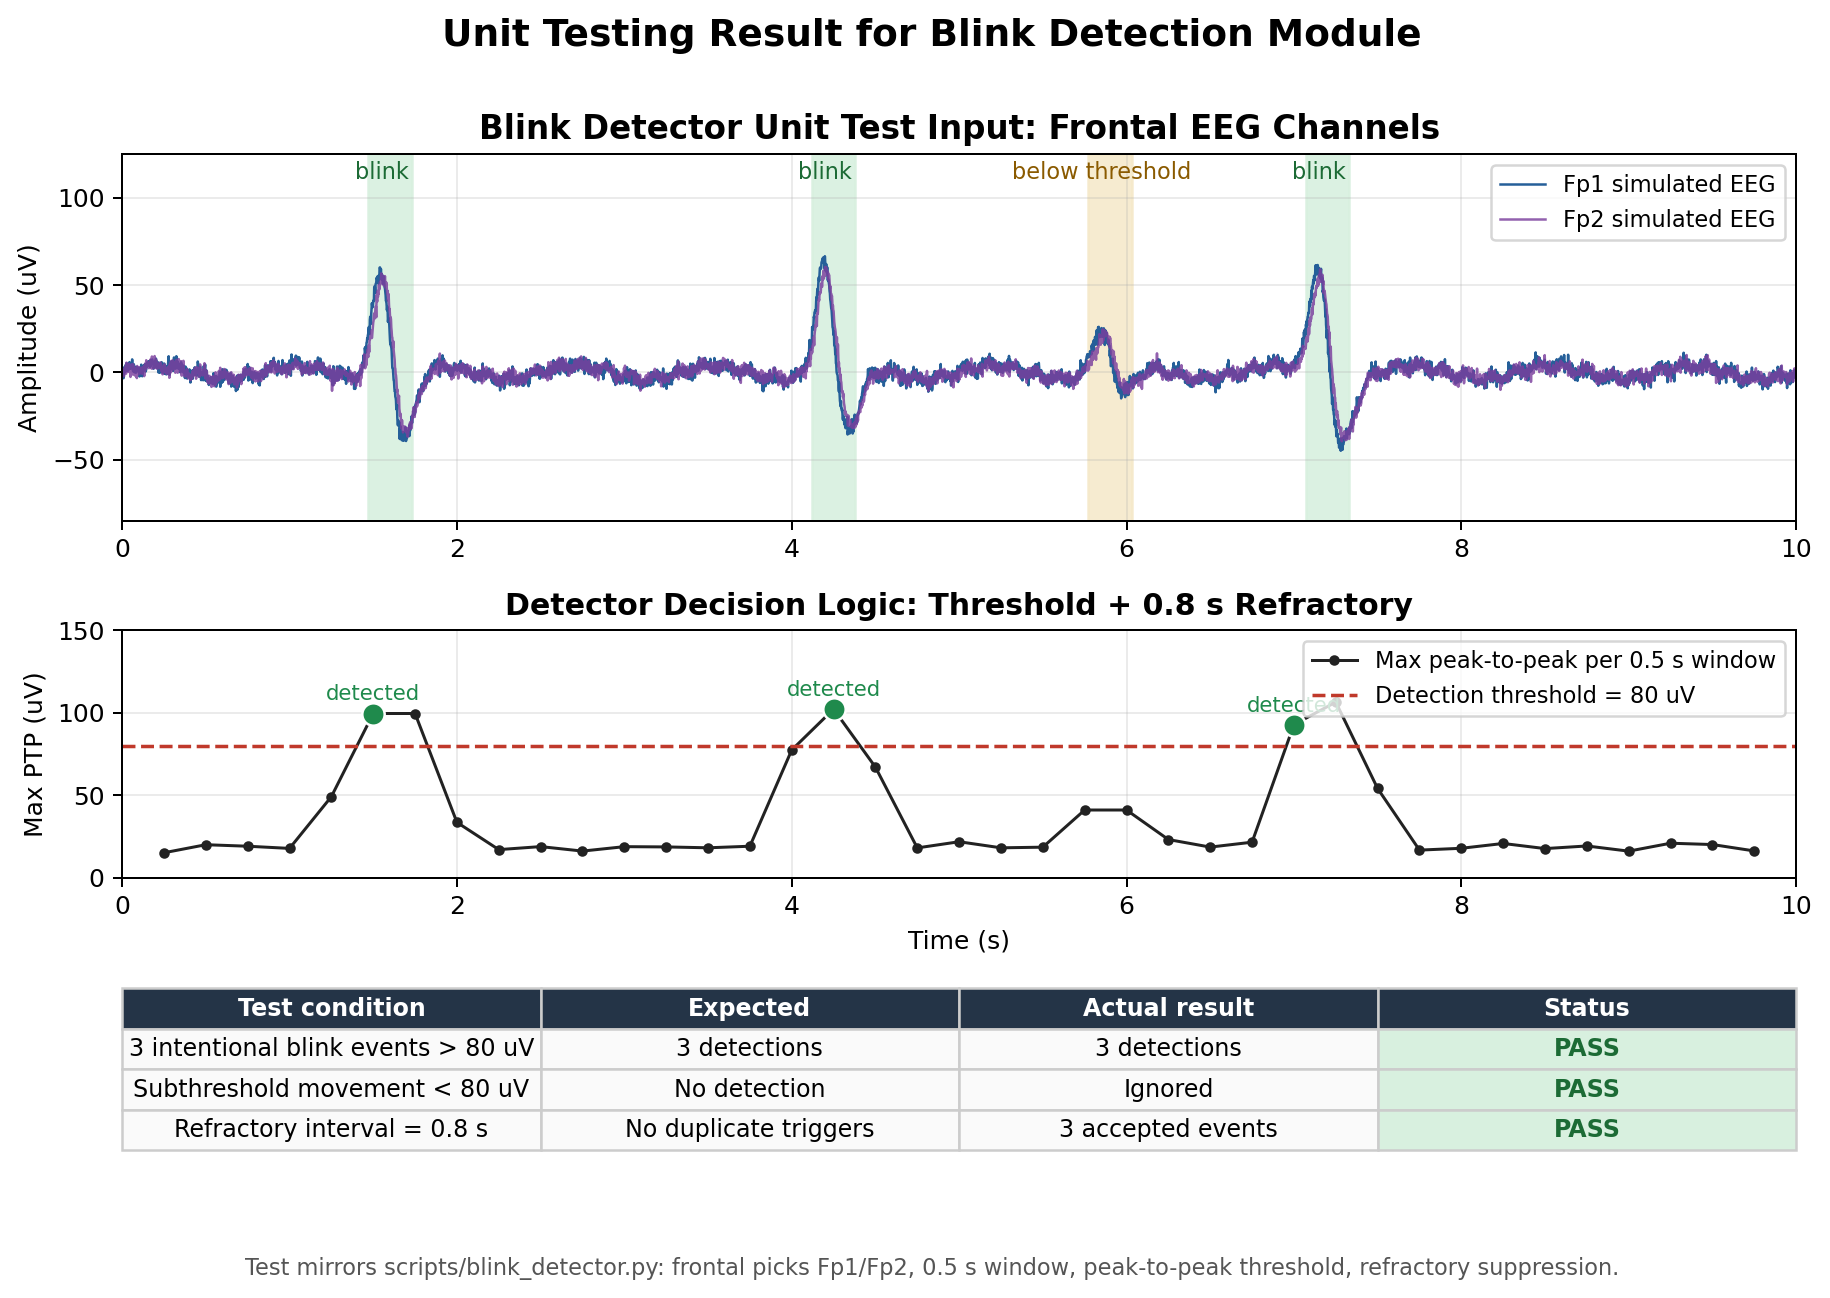
\includegraphics[width=\linewidth,height=0.72\textheight,keepaspectratio]{images/blink_test.png}
    \caption{Unit Testing Results for Blink Detection Module}
    \label{fig:blink_test}
\end{figure}

\subsection{System Performance Testing}

The available saved models and datasets were evaluated from the current repository snapshot. The term \textit{saved-model accuracy} refers to the accuracy of an already trained \texttt{.joblib} model when evaluated on the corresponding available recorded epochs. These values are useful for reporting model behavior on the available data, but they can be optimistic if the same epochs were used during model training. Therefore, 5-fold cross-validation is also reported where complete subject epoch/label files are available.

\subsubsection{Saved-Model Accuracy on Available Datasets}

\begin{table}[H]
    \centering
    \caption{Saved FBCSP+LDA Model Accuracy on Matching Available Datasets}
    \label{tab:saved_model_accuracy}
    \resizebox{\textwidth}{!}{%
    \begin{tabular}{|l|l|c|c|c|}
        \hline
        \textbf{Model} & \textbf{Evaluation Dataset} & \textbf{Trials} & \textbf{Saved-Model Accuracy} & \textbf{Notes} \\ \hline
        \texttt{fbcsp\_lda\_S02.joblib} & S02 & 160 & 70.0\% & Matching subject data \\ \hline
        \texttt{fbcsp\_lda\_S12.joblib} & S12\_U & 20 & 100.0\% & Closest available S12 dataset \\ \hline
        \texttt{fbcsp\_lda\_S14\_U.joblib} & S14\_U & 20 & 100.0\% & Matching subject data \\ \hline
        \texttt{fbcsp\_lda\_S15.joblib} & S15 & 40 & 100.0\% & Matching subject data \\ \hline
        \texttt{fbcsp\_lda\_S20.joblib} & S20 & 40 & 95.0\% & Matching subject data \\ \hline
        \texttt{fbcsp\_lda\_S21.joblib} & S21 & 40 & 97.5\% & Matching subject data \\ \hline
        \texttt{fbcsp\_lda\_from\_npz.joblib} & raw\_012\_4s & 160 & 82.5\% & Raw NPZ channels 0,1,2; 4s \\ \hline
        \texttt{fbcsp\_lda\_from\_npz\_012\_3s.joblib} & raw\_012\_3s & 160 & 83.8\% & Raw NPZ channels 0,1,2; 3s \\ \hline
        \texttt{fbcsp\_lda\_from\_npz\_012\_4s.joblib} & raw\_012\_4s & 160 & 82.5\% & Raw NPZ channels 0,1,2; 4s \\ \hline
        \texttt{fbcsp\_lda\_from\_npz\_034\_3s.joblib} & raw\_034\_3s & 160 & 94.4\% & Raw NPZ channels 0,3,4; 3s \\ \hline
    \end{tabular}%
    }
\end{table}

The 100\% saved-model accuracies for some small datasets should be interpreted carefully because they are loaded-model evaluations on limited same-session calibration data. The cross-validation results below provide a more conservative estimate.

\subsubsection{Five-Fold Cross-Validation on Available Subject Datasets}

\begin{table}[H]
    \centering
    \caption{Five-Fold Cross-Validation Accuracy on Available Subject Epoch Files}
    \label{tab:cv_accuracy}
    \resizebox{\textwidth}{!}{%
    \begin{tabular}{|l|c|c|c|c|}
        \hline
        \textbf{Subject Dataset} & \textbf{Trials} & \textbf{Saved-Model Accuracy} & \textbf{5-Fold CV Mean} & \textbf{5-Fold CV Std Dev} \\ \hline
        S02 & 160 & 70.0\% & 61.9\% & 5.4\% \\ \hline
        S11 & 50 & N/A & 48.0\% & 9.8\% \\ \hline
        S12\_U & 20 & 100.0\% & 70.0\% & 18.7\% \\ \hline
        S14\_U & 20 & 100.0\% & 75.0\% & 15.8\% \\ \hline
        S15 & 40 & 100.0\% & 82.5\% & 10.0\% \\ \hline
        S20 & 40 & 95.0\% & 75.0\% & 11.2\% \\ \hline
        S21 & 40 & 97.5\% & 87.5\% & 7.9\% \\ \hline
    \end{tabular}%
    }
\end{table}

\textbf{Note:} Cross-validation retrains the FBCSP+LDA pipeline inside each fold and is therefore a better indicator of generalization than saved-model accuracy on the full calibration set. The S11 dataset has no saved model in the current repository but was included in CV because its epochs and labels are available.

\subsubsection{Proxy Evaluation for Models Without Matching Archived Data}

Some saved subject models do not have their original matching epoch/label files in the current repository snapshot. These models were evaluated on the best available compatible dataset only as proxy/cross-dataset checks. They should not be reported as true subject-specific accuracy.

\begin{table}[H]
    \centering
    \caption{Proxy Best-Available Evaluation for Models Without Matching Subject Data}
    \label{tab:proxy_accuracy}
    \resizebox{\textwidth}{!}{%
    \begin{tabular}{|l|l|c|c|}
        \hline
        \textbf{Model} & \textbf{Proxy Dataset} & \textbf{Trials} & \textbf{Proxy Accuracy} \\ \hline
        \texttt{fbcsp\_lda\_S03.joblib} & raw\_034\_3s & 160 & 66.2\% \\ \hline
        \texttt{fbcsp\_lda\_S04.joblib} & S15 & 40 & 60.0\% \\ \hline
        \texttt{fbcsp\_lda\_S05.joblib} & S20 & 40 & 57.5\% \\ \hline
        \texttt{fbcsp\_lda\_S06.joblib} & raw\_012\_4s & 160 & 63.7\% \\ \hline
        \texttt{fbcsp\_lda\_S07.joblib} & S15 & 40 & 67.5\% \\ \hline
        \texttt{fbcsp\_lda\_S08.joblib} & S21 & 40 & 62.5\% \\ \hline
        \texttt{fbcsp\_lda\_S10.joblib} & S20 & 40 & 55.0\% \\ \hline
    \end{tabular}%
    }
\end{table}

\subsection{Confusion Matrix Analysis}

The FBCSP+LDA classifier was evaluated on the binary task Rest (class 0) versus Motor Imagery (class 1). A representative high-performing primary saved-model evaluation is shown for S21. The model correctly classified 39 out of 40 trials, producing an overall saved-model accuracy of 97.5\%.

\begin{table}[H]
    \centering
    \caption{Confusion Matrix for Subject S21 Saved Model - Binary Classification (Rest vs. Motor Imagery)}
    \label{tab:confusion_s21}
    \begin{tabular}{|l|c|c|c|}
        \hline
        \textbf{True/Predicted} & \textbf{Rest (Class 0)} & \textbf{Motor Imagery (Class 1)} & \textbf{Recall} \\ \hline
        \textbf{Rest (Class 0)} & 20 & 0 & 100.0\% \\ \hline
        \textbf{Motor Imagery (Class 1)} & 1 & 19 & 95.0\% \\ \hline
        \textbf{Precision} & 95.2\% & 100.0\% & \textbf{97.5\% Overall} \\ \hline
    \end{tabular}
\end{table}

For comparison, the S02 saved model produced the following confusion matrix: Rest $=58$ correct and $22$ misclassified as Motor Imagery; Motor Imagery $=54$ correct and $26$ misclassified as Rest, giving an overall accuracy of 70.0\%.

\textbf{Important:} Blink detection is implemented as a separate threshold-based detector and is not included in the FBCSP+LDA confusion matrices. Blink events are detected using peak-to-peak amplitude thresholding on frontal EEG channels, whereas the matrices above evaluate only Rest versus Motor Imagery.

\begin{figure}[H]
    \centering
    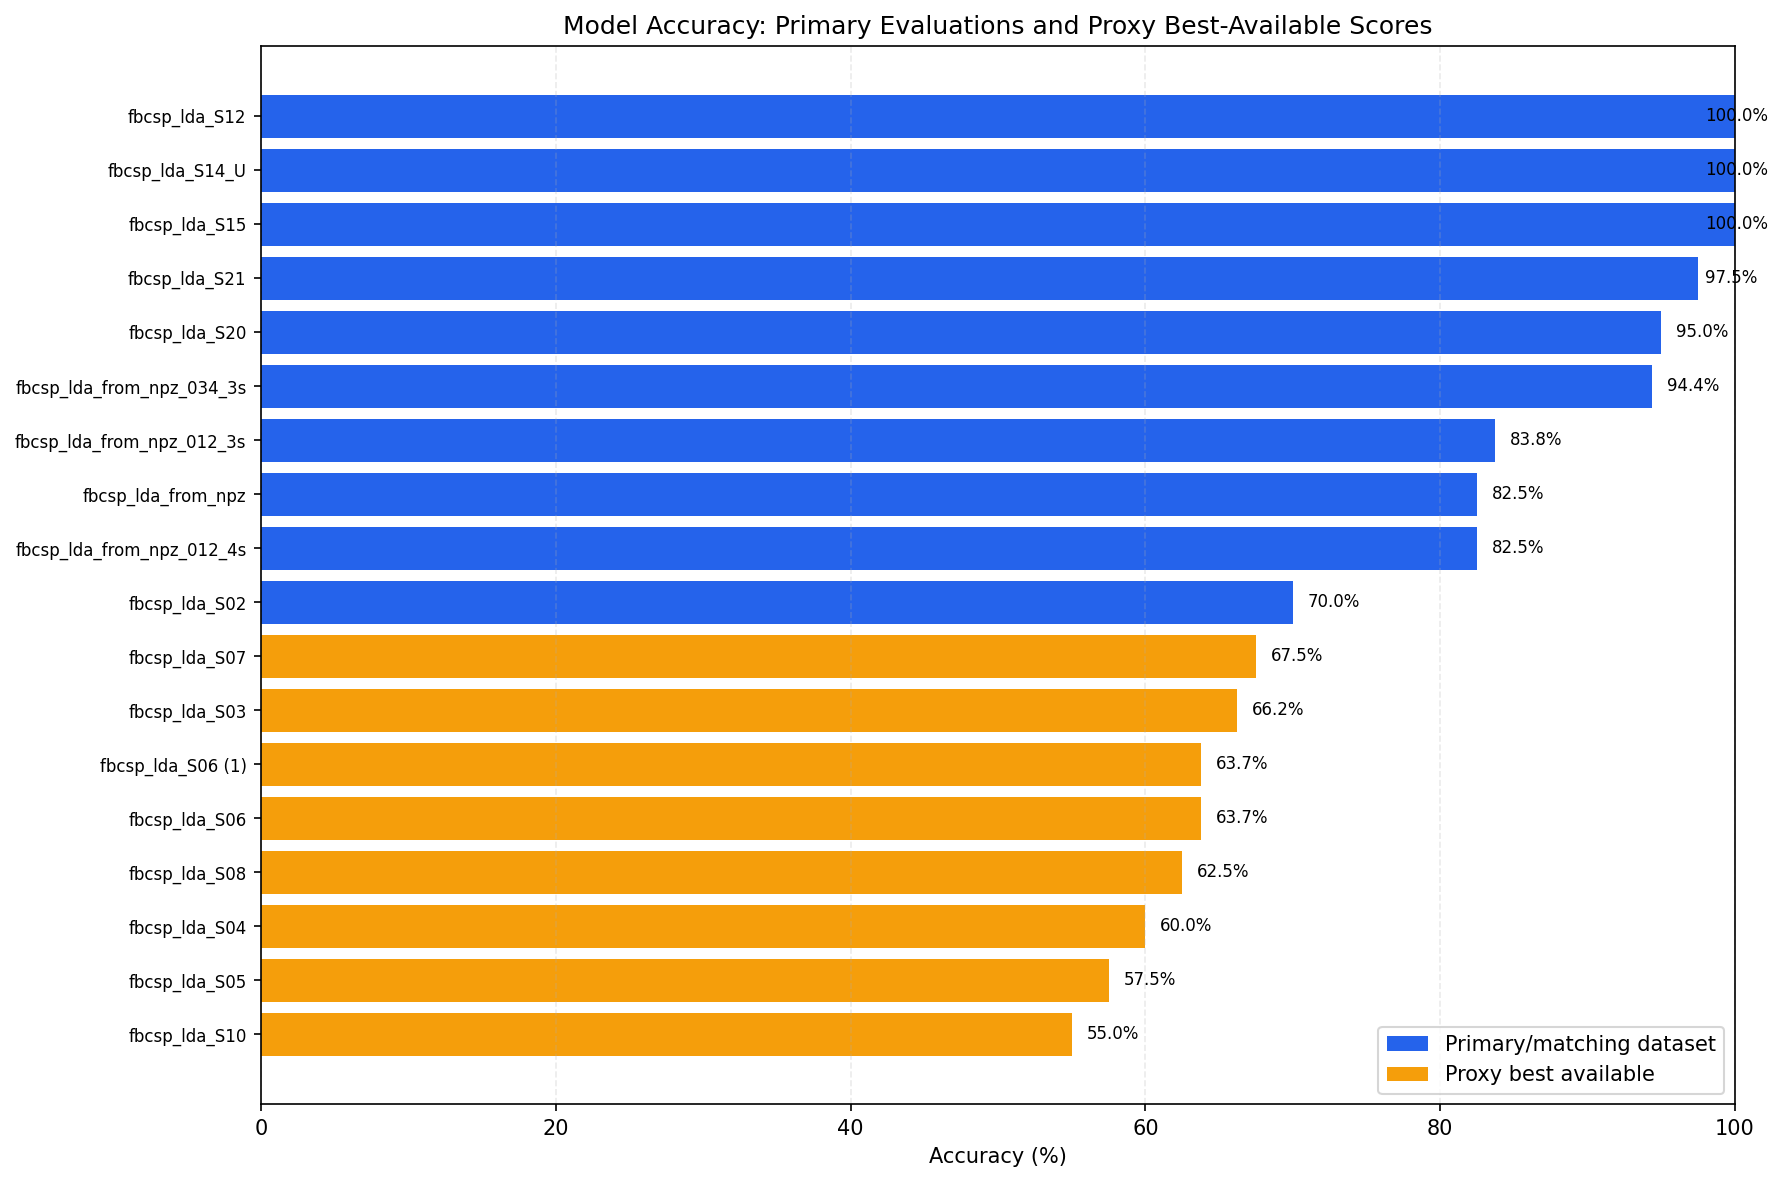
\includegraphics[width=0.92\linewidth,height=0.58\textheight,keepaspectratio]{reports/figures/model_accuracy_bar.png}
    \caption{Saved-Model Accuracy Summary for Primary and Proxy Evaluations}
    \label{fig:model_accuracy_bar}
\end{figure}

\begin{figure}[H]
    \centering
    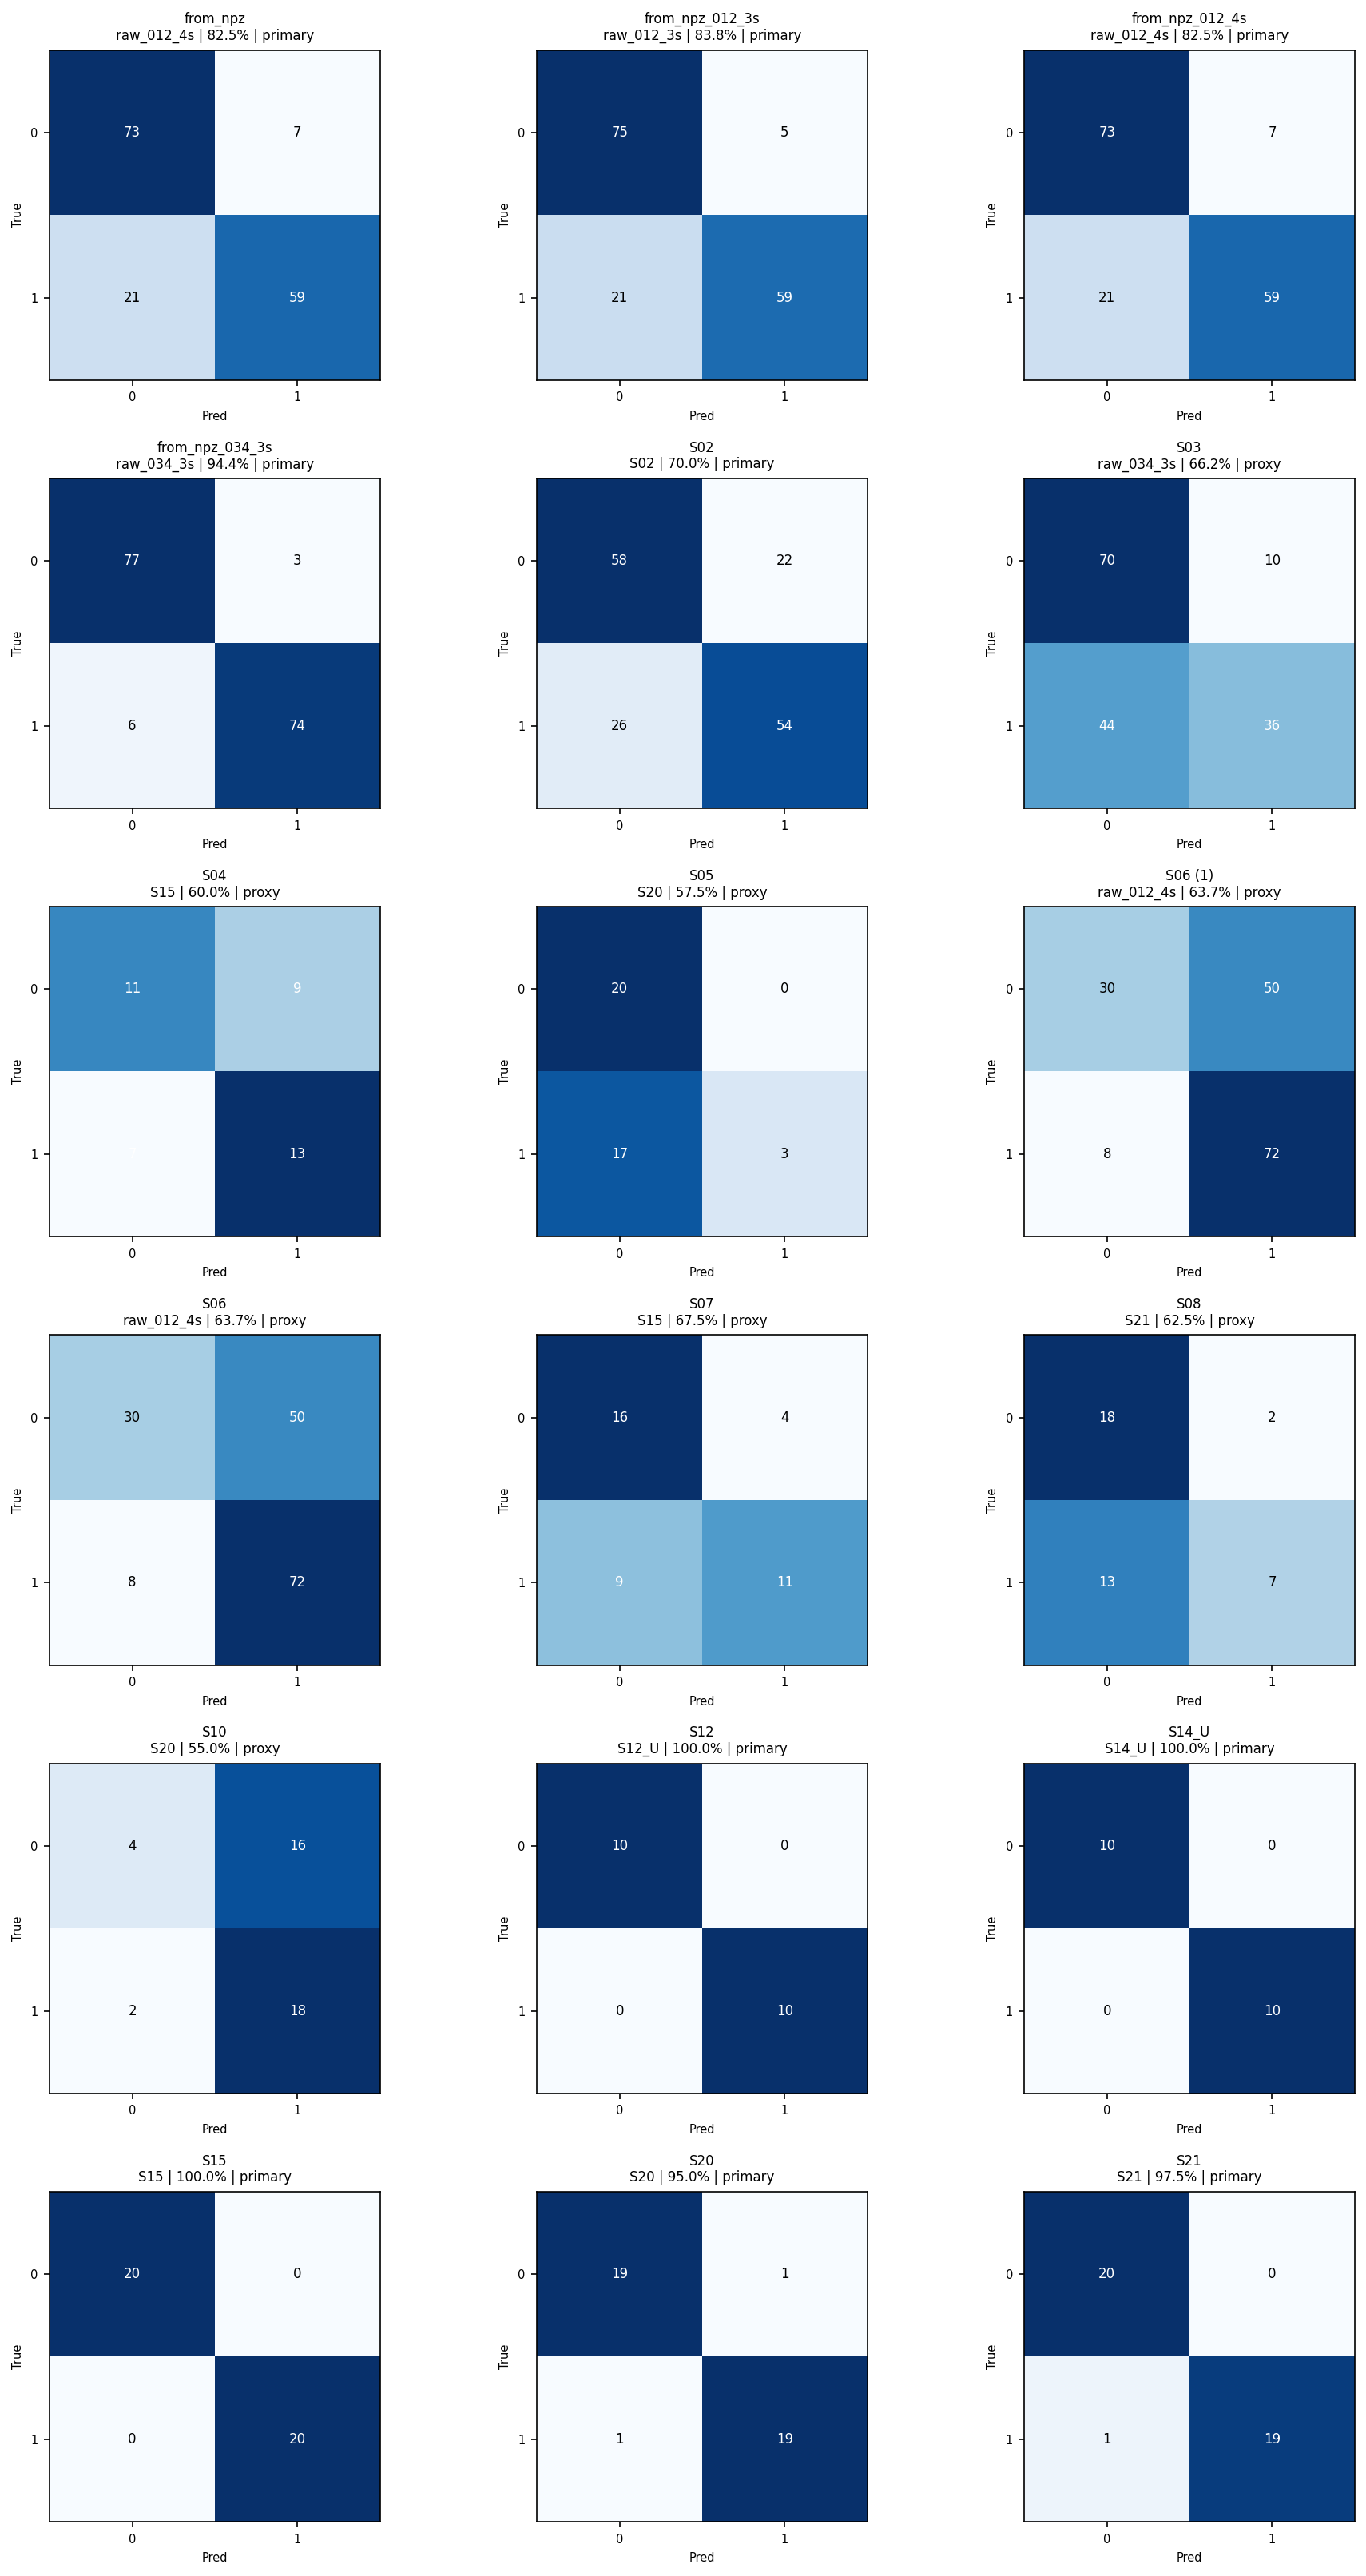
\includegraphics[width=0.92\linewidth,height=0.58\textheight,keepaspectratio]{reports/figures/selected_confusion_matrices_grid.png}
    \caption{Selected Confusion Matrices for Evaluated Models}
    \label{fig:confusion_grid}
\end{figure}

\subsection{Latency Benchmarking}

The real-time classifier uses a 4-second EEG window with a 0.5-second sliding step at 500 Hz. Therefore, the overall user-intent-to-decision time is dominated by the window acquisition requirement, not by the classifier computation itself.

\subsubsection{Window Acquisition Latency}

\begin{itemize}
    \item \textbf{Window Length:} 4.0 seconds of EEG data
    \item \textbf{Sliding Step:} 0.5 seconds
    \item \textbf{Sampling Rate:} 500 Hz per channel
    \item \textbf{Samples per Window:} 2000 samples per channel
\end{itemize}

This means the first classification decision requires approximately 4 seconds of data. After the first window is available, the classifier can update every 0.5 seconds using overlapping windows. This design is suitable for slower or turn-based gameplay, but it is not ideal for fast action games requiring instant responses.

\subsubsection{Post-Window Processing Latency}

Once a complete EEG window is available, post-window computation consists of bandpass filtering, CSP projection, log-variance feature extraction, LDA prediction, and command emission. The generated evaluation data in this repository focuses on classification accuracy and confusion matrices; therefore, subject-specific latency tables should only be included if separate timing logs are available. Without timing logs, the most defensible statement is that the design updates every 0.5 seconds after the initial 4-second buffer is filled.

\subsection{Runtime Resource Utilization}

The implementation is lightweight and runs without GPU acceleration. CPU and memory usage depend on the number of active modules, including the GUI, LSL acquisition, blink detector, gyroscope detector, and game overlay. Since no formal resource log is archived with the current evaluation data, resource figures should be reported as implementation observations unless measured with a profiler during a controlled session.

\subsection{Limitations and Error Analysis}

The following limitations were identified from implementation behavior and the available evaluation data:

\begin{enumerate}
    \item \textbf{Saved-Model Accuracy vs. Generalization:} Saved-model accuracy can be high when evaluated on the same calibration/session data used during training. Cross-validation results are more conservative and should be emphasized for generalization claims.
    \item \textbf{Small Dataset Sizes:} Some subject datasets contain only 20 or 40 trials. Perfect saved-model scores on these datasets should be interpreted cautiously.
    \item \textbf{Missing Original Data for Some Models:} Models S03, S04, S05, S06, S07, S08, and S10 do not have their matching archived subject datasets in the current repository snapshot, so their reported proxy scores are not true subject accuracies.
    \item \textbf{Subject Variability:} Cross-validation scores vary across subjects, ranging from 48.0\% for S11 to 87.5\% for S21, indicating strong subject-dependent differences in motor imagery separability.
    \item \textbf{Window-Based Latency:} The 4-second analysis window improves signal stability but increases the time before the first decision can be made.
    \item \textbf{Artifact Sensitivity:} Eye blinks and muscle activity can contaminate motor imagery features. The blink detector is separated from the FBCSP+LDA classifier to reduce confusion between blink events and MI/rest classification.
    \item \textbf{Limited Command Vocabulary:} The current binary EEG classifier supports Rest and Motor Imagery. Additional commands would require more training data, additional paradigms, more channels, or alternative models.
\end{enumerate}

Overall, the available results show that the implemented FBCSP+LDA pipeline can classify binary motor imagery from recorded EEG data, with saved-model accuracies reaching 70.0\% to 100.0\% on matching available datasets and cross-validation scores reaching up to 87.5\%. These results support the feasibility of the system while also showing the need for careful reporting, larger datasets, and held-out testing for stronger generalization claims.
